\documentclass[12pt]{article}
\usepackage[left=3.5cm,right=2cm,top=2.5cm,bottom=2.5cm]{geometry}
\usepackage[T1]{fontenc}
\usepackage[utf8]{inputenc}
\usepackage{tgpagella}
\usepackage{enumerate}
\usepackage{url}
\usepackage{multirow}
\usepackage{longtable}
\usepackage{polski}
\usepackage{graphicx}
\usepackage{float}
\usepackage{color}
\usepackage{amsmath}
\usepackage{longtable}
\usepackage{tabularx}
\usepackage{ltablex,booktabs}
\usepackage{amssymb}
\usepackage{rotating}
\usepackage{subfigure}
\usepackage{float}
\usepackage{tabu}
\usepackage{caption}
\usepackage{footnote}
\usepackage{xspace}
\usepackage{mathpazo}
\usepackage[table]{xcolor}
\usepackage[justification=centering]{caption}
\graphicspath{ {images/} }

\pagestyle{empty}

\title{\LARGE{Uniwersytet Wrocławski}\\
\Large{Wydział Matematyki i Informatyki}\\
\large{Kierunek: Informatyka}}

\date{}

\begin{document}
\pagestyle{empty}

\begin{titlepage}
\maketitle
\thispagestyle{empty}


\begin{center}
\author{\LARGE{Adrian Mularczyk}}
\vspace{30pt}

\huge{\textbf{Stworzenie wydajnego wzorca wstrzykiwania zależności dla złożonych grafów zależności}}
\vspace{50pt}
\end{center}

\begin{flushright}
\large{Praca wykonana pod kierunkiem}
\large{dr. Wiktora Zychli}
\end{flushright}

\vfill
\begin{center}
\begin{large}
Wrocław, 2016
\end{large}
\end{center}
\end{titlepage}

\setlength{\parindent}{0pt}	%usunięcie wcięć
\setlength{\parskip}{1.5ex} 
\renewcommand*{\figurename}{Rys.}
\renewcommand*{\tablename}{Tab.} 
\renewcommand{\captionsize}{\small}


\clearpage

\tableofcontents



\clearpage

\section{Wstęp}
\subsection{Cel pracy}
Wstrzykiwanie zależnośc jest wzorcem projektowym, który pozwala na tworzenie kodu o luźniejszych powiązaniach, łatwiejszego w testowaniu i modyfikacji. Najbardziej popularnymi implementacjami tego wzorca w języku C\# są Unity i Ninject. Celem niniejszej pracy magisterskiej jest stworzenie wydajnej implementacji tego wzorca dla złożonych grafów zależności. Do tego celu zostanie wykorzystana funkcjolanosci z przestrzeni nazw Reflection.Emit. W tej pracy zostaną przedstawione dwa rozwiązania.

\subsection{Układ pracy}
Poza wstępem i podsumowaniem praca składa się jeszcze z trzech rozdziałów. W pierwszym znajduje się opis teoretyczny czym jest wstrzykiwanie zależności. Drugi rozdział opisuje moją implementację tego wzorca. Trzeci rozdział skupia się na testach wydajnościowych, w którym porównuję moją implementację z kilkoma najbardziej popularnym i kilkoma najszybszymi implementacjami.



\clearpage

\section{Wstrzykiwanie zależnosci}
\subsection{Wstęp}
Jest to zbiór zasad projektowania oprogramowania i wzorców, które pozwalają nam rozwijać luźno powiązany kod.\\
Jakiemu celowi ma służyć wstrzykiwanie zależności? Wstrzykiwanie zależnści nie jestem celem samym w sobie, raczej jest to środek do celu. Ostatecznie celem większości technik programowania jest dostarczenie jak najwydajniej działającego oprogramowania. Jednym z aspektów tego jest napisanie utrzymywalnego kodu.\\
O ile nie pisze się prototypu lub aplikacji, które nigdy nie mają kolejnych wersji (kończą się na wersji 1), to wkrótce będzie trzeba zająć się utrzymaniem i rozwijaniem istniejącego kodu. Aby być w stanie pracować wydajnie z takim kodem bazowym, musi on być jak najlepiej utrzymywalny.\\
Wstrzykiwanie zależności jest niczym więcej niż techniką, która umożliwia luźne powiązania, a luźne powiązania sprawiają, że kod jest rozszerzalny i łatwy w utrzymaniu.\cite{dependency_injection}\\
Wstrzykiwanie zależności może odbywać się na 3 sposoby:
\begin{itemize}
	\item wstrzykiwanie przez konstruktor
	\item wstrzykiwanie przez metodę
	\item wstrzykiwanie przez właściwość
\end{itemize}

\subsubsection{Wstrzykiwanie przez konstruktor}
\begin{figure}[h]
	\begin{raggedleft}
  		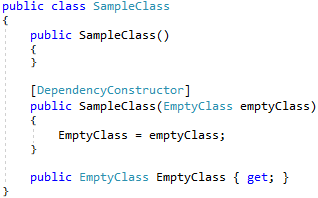
\includegraphics{DependencyConstructor.png}
	\end{raggedleft}
\end{figure}
Jest to główny i najbardziej popularny sposób wstrzykiwania zależności. Niektóre klasy mają kilka konstruktor i atrybut "DependencyConstructor" przydaje się wtedy do oznaczenia, który z nich ma zostać wybrany przy tworzeniu nowego obiektu. Jednakże nie zawsze jest on potrzebny. W większości przypadków klasy mają tylko jeden konstruktor, a także rozwiązania przemsysłowe mają logikę, która wybierze odpowiedni konstruktor (np. ten oznaczony atrybutem, albo ten co ma najwięcej parametrów, albo ten co ma najmniej parametrów).

\subsubsection{Wstrzykiwanie przez metodę}
\begin{figure}[h]
	\begin{raggedleft}
  		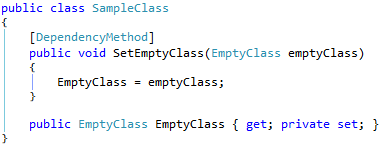
\includegraphics{DependencyMethod.png}
	\end{raggedleft}
\end{figure}
W przemysłowych rozwiązaniach to wstrzykiwanie z reguły odbywa się albo poprzez oznaczenie metody przez którą chcemy wstrzyknąć zaleźności odpowiednim atrybutem, albo przy rejestracji danej klasy definijumey przez jakie metody chcemy wstrzyknąć zależności.

\subsubsection{Wstrzykiwanie przez właściwość}
\begin{figure}[h]
	\begin{raggedleft}
  		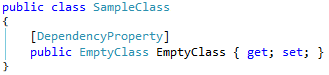
\includegraphics{DependencyProperty.png}
	\end{raggedleft}
\end{figure}
Tutaj podobnie jak dla wstrzykiwania przez metodę w przemysłowych rozwiązaniach to wstrzykiwanie z reguły odbywa się albo poprzez oznaczenie właściwoci przez którą chcemy wstrzyknąć zaleźności odpowiednim atrybutem, albo przy rejestracji danej klasy definijumey przez jakie właściwości chcemy wstrzyknąć zależności.


\clearpage
\subsection{Implementacje przemysłowe}
Na rynku jest wiele implementacji wstrzykiwania zależności. Przedstawię tutaj kilka najbardziej popularnych (według ilości pobrań z NuGet) oraz kilka najszybszych (według rankingu na stronie: http://www.palmmedia.de/Blog/2011/8/30/ioc-container-benchmark-performance-comparison). Dane zostały wzięte z dnia 21-02-2017. W nawiasie znajduje się wersja implementacji, która została użyta w testach (najnowsza na ten dzień).\\
\\
Najbardziej popularne:
\begin{itemize}
	\item Unity (4.0.1) - ponad 5.2 mln pobrań
	\item NInject (3.2.2) - ponad 4.0 mln pobrań
	\item Autofac (4.3.0) - ponad 3.7 mln pobrań
	\item StructureMap (4.4.3) - ponad 1.6 mln pobrań
	\item Windsor (3.4.0) - ponad 1.4 mln pobrań
\end{itemize}
Najszybsze:
\begin{itemize}
	\item Grace (5.1.0)
	\item DryIoc (2.10.1)
	\item LightInject (5.0.1)
	\item SimpleInjector (3.3.2)
\end{itemize}



\clearpage
\section{Implementacja}
Kod źródłowy programu jest dostępnym w repozytorium pod adresem:\\
\url{https://github.com/amularczyk/NiquIoC}\\
Znajduje się tam również kod programu, który posłużył do wykonania testów wydajnościowych, a także ta praca napisana w języku LateX i wszystkie obrazki.

\subsection{Środowisko pracy}
Prac oraz wszystkie testy powstały na komputerze z parametrami:
\begin{itemize}
	\item Intel Core i7-4720HQ (2.60GHz)
	\item 12 GB pamięci RAM
	\item Dysk SSD
\end{itemize}
Narzędzia użyte do stworzenia pracy i testów:
\begin{itemize}
	\item System operacyjny Windows 10 Pro
	\item .Net Framework w wersji 4.6.1
	\item Visual Studio 2017 Comunnity
	\item MSTest
	\item ReSharper
	\item dotCover
	\item Dia
\end{itemize}


\subsection{Wstęp}
Na początku chciałbym pokrótce opisać dwie rzeczy, które są istotne dla mojego rozwiązania. Pierwszą z nich jest Microsoft Intermediate Language, a drugą przestrzeń nazw Reflection.Emit.

\subsubsection{Microsoft Intermediate Language}
Microsoft Intermediate Language - MSIL (w skrócie IL) to język pośredni do którego kod C\# jest kompilowany. Język ten pozwala na komunikację między aplikacjami napisanymi na platformie .Net, a systemem operacyjnym. Jest on jądrem tej platformy.

\subsubsection{Reflection.Emit}
Przestrzeń nazw Reflection.Emit pozwala w języku C\# na stworzenie ciągu operacji w języku IL, a następnie zapamiętaniu ciągu tych operacji jako delegat. Za każdym razem, gdy ten delegat zostanie wywołany, to wykona się ciąg wczeniej zdefiniowanych operacji IL.


\subsection{Opis}
Aplikacja składa się z 1 projektu i 8 projektów na potrzeby testów. Rozwiązanie jest skomplikowana i aby mieć pewność, że działa w pełni dobrze zostało stworzone  ponad 1200 testów jednostkowych, a pokrycie kodu testami wynosi ponad 97\%.\\

W wykonanej implementacji został stworzony interfejs IConatiner, który definiuje operacje, jakie powinny się znaleźć w każdym kontenerze:
\begin{figure}[h]
	\begin{raggedleft}
  		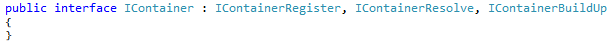
\includegraphics{IContainer.png}
	\end{raggedleft}
\end{figure}\\
Pierwsze cztery metody służą do rejestracji typów w kontenerze. Metoda piąta (Resolve) służy do tworzenia i zwracania obiektów wczeniej zarejestrowanych typów. Ostatnia metoda (BuildUp) do uzupełnienia istniejącej istancji obiektu z wykorzystaniem wstrzykiwania zależności przez metodę i właściwość - jest to metoda opcjonalna i nie każde przemysłowe rozwiązanie ją zawiera.\\
Poniżej znajduje się dokładniejszy opis każdej z metod.

\clearpage
\subsubsection{Register}
W pierwszej metodzie możemy zarejestrować zwykłe klasy. W drugiej interfejsy i klasy, które implementują dany interfejs lub klasy i klasy po nich dziedziczące. W trzeciej metodzie rejestrujemy klasę jako fabrykę obiektów - funkcję, która ma nam zwrócić pożądany obiekt. W czwartej natomiast możemy zarejestrować konkretną instancję danego typu.\\
W moim rozwiązaniu każdy typ może być zarejestrowany tylko raz - ponowna rejestracja tego samego typu nadpisuje istniejącą rejestrację.\\
Każda z tych czterech metod rejestracji zwraca interfejs IContainerMember, który umożliwia nam zarejestrowanie danego typu z określonym menadżerem czasu życia (czyli implementacją interfejsu IObjectLifetimeManager). Jest to po to, ponieważ dla różnych przypadków biznesowych możemy potrzebować, aby obiekt danego typu miał konretny czas życia. Interfejs IContainerMember wygląda następująco:
\begin{figure}[h]
	\begin{raggedleft}
  		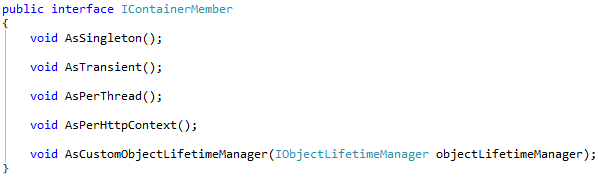
\includegraphics{IContainerMember.png}
	\end{raggedleft}
\end{figure}\\
Pierwsze cztery metody tego interfejsu to wbudowane implementacje interfejsu IObjectLifetimeManager. Piąta metoda dostarcza możliwoć podania przez użytkownika jego własnej implementacji tego interfejsu. W moim rozwiązaniu każdy typ domyślnie ma czas życia Transient.\\
\\
Wyjaśnienie rozdajów czasu życia:
\begin{itemize}
	\item Singleton - za każdym razem zwracany jest ten sam obiekt
	\item Transient - za każdym razem zwracany jest nowy obiekt
	\item PerThread - wewnątrz danego wątku zwracany jest ten sam obiekt, ale dla innego wątku zwracany jest nowy (inny) obiekt
	\item PerHttpContext - wewnątrz danego żądania Http zwracany jest ten sam obiekt, ale dla innego żądania zwracany jest nowy (inny) obiekt
\end{itemize}

\clearpage
Interfejs IObjectLifetimeManager prezentuje się tak:
\begin{figure}[h]
	\begin{raggedleft}
  		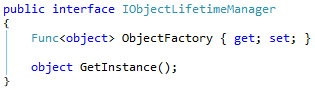
\includegraphics{IObjectLifetimeManager.png}
	\end{raggedleft}
\end{figure}\\
Właściwość ObjectFactory służy do ustawienia funkcji, która zwraca obiekt. Metoda GetInstance służy do pobrania obiektu.\\
W zależności od implementacji tego interfesju, to obiekt zwracany z metody GetInstance może być zawsze taki sam, zawsze różny albo taki sam tylko dla określonych sytuacji (np. taki sam dla tego samego wątku albo tego samego żądania http).

\subsubsection{Resolve}
Metoda piąta - Resolve, jest to główna operacja. Register można nazwać sercem kontenera, a Resolve mózgiem. Odpowiada ona za stworzenie i zwrócenie obiektu odpowiedniego typu.\\
W mojej pracy zaproponowałem dwa rozwiązania - PartialEmitFunction i FullEmitFunction, dlatego ta metoda jako parametr przyjmuje wartość enuma ResolveKind (dzięki temu w przyszłości może być ona w łatwy sposób rozszerzona o kolejne rozwiązania).

\subsubsection{BuildUp}
Szósta metoda to taki dodatek - gdy mamy stworzony obiekt, ale nie jest w pełni uzupełniony, wtedy możemy go zbudować (używająć odpowiedniej wartości z enuma ResolveKind). Z tą metodą są powiązane bezpośrednio dwa pojęcia - wstrzykiwanie przez metodę i wstrzykiwanie przez właściwość. Do tego celu w moim rozwiążaniu stworzyłem dwa atrybuty:
\begin{itemize}
	\item DependencyMethod (dla metod)
	\item DependencyProperty (dla właściwości)
\end{itemize}
Podczas operacji BuildUp wywoływane są wszystie metody i uzupełniane są wszystkie właściwości, które mają te atrybuty. Ta operacja jest również wykonywany podczas operacji Resolve.\\

Warto tutaj odnotować, że ze względu na szczegóły implementacyjne tylko jedno z moich rozwiązań wspiera operację BuildUp - jest to rozwiązanie PartialEmitFunction. W rozwiązaniu FullEmitFunction ta funckonalność nie została zaimplementowana. Jest to spowodowane skomplikowaniem tego rozwiązania i małą potrzebą biznesową używania tej operacji. Jednakże w przyszłości istnieje możliwość dodania implementacji tej funkcjonalności.\\

W aplikacji istnieje również atrybut DependencyConstrutor. Można go użyć przy definicji konstruktora danej klasy. Obiekt każdej klasy jest tworzony przy użyciu konstruktora. Klasa może mieć kilka konstruktorów. W moim rozwiązaniu stworzyłem logikę wyboru odpowiedniego konstruktora, przy pomocy którego ma zostać stworzony obiekt. Wygląda ona następująco:
\begin{itemize}
	\item Jeśli jest jeden konstruktor, to go wybierz.
	\item Jeśli jest kilka konstruktorów, to odpowiedni wybierz w poniższej kolejności:
	\begin{enumerate}
		\item Konstruktor z atrybutem DependencyConstrutor
		\item Konstruktor z największą liczbą parametrów
	\end{enumerate}
	\item Jeśli jest kilka konstrutkrów z atrybutem DependencyConstrutor albo nie ma żadnego konstruktora z tym atrybutem i jest kilka z największą liczbą parametrów, to rzuć wyjątek.
\end{itemize}


\subsection{Rozwiązanie}
Stworzenie nowego obiektu zajmuje czas. Gdy graf zależności dla jakiegoś typu jest bardzo rozbudowany, to stworzenie takiego obiektu zajmuje dużo czasu. Proces ten można podzielić na trzy etapy:
\begin{itemize}
	\item Uzyskanie informacji obiekty jakich typów są potrzebne do stworzenia danego obiektu.
	\item Stworzenie tych pomocnicznych obiektów.
	\item Stworzenie docelowego obiektu.
\end{itemize}
Gdy mamy rozbudowane grafy zależności, to często zdaża się, że niektóre typy się powtarzają. Zatem pewne informacje możemy uzyskać raz, a następnie je zapamiętać. Aby implementacja wzorca wstrzykiwania zależności działała wydajnie dla złożonych grafów zależności, należy jak najwięcej informacji przechowywać w pamięci podręcznej i należy to robić mądrze.\\
W mojej implementacji stworzyłem dwie strategie, które realizują te założenia. W pierwszym rozwiązaniu zapamiętuje każdy z tych 3 puntków osobno, a w drugim rozwiązaniu zapamiętuję wszystko na raz. Do zapamiętania kroków potrzebnych do stworzenia obiektu danego typu wykorzystałem operacje z przestrzeni nazw Reflection.Emit.

\subsubsection{Rozwiązanie 1 - PartialEmitFunction}
Pierwsze rozwiązanie nazwałem PartialEmitFunction, ponieważ cały process tworzenia nowego obiektu został rozbity na mniejsze części (docelowy obiekt tworzę po kawałku).\\

Tworzę w nim delegata z wykorzystaniem Reflection.Emit. Delegat ten jako parametr przyjmuje listę obiektów, które są potrzebne do stworzenia obiektu danej klasy wykorzystując odpowiedni konstruktor. Jeśli kontener do stworzenia obiektu danej klasy wybrał konstruktor bezparametrowy, to do takiego delegata trafi pusta lista. Jeśli natomiast został wybrany konstruktor, który w parametrze przynmuje obiekty jakiś typów, to lista tych obiektów w odpowiedniej kolejności zostanie przekazana do delegata (np. obiekt, który chcemy stworzyć w konstrutkorze który został wybrany potrzebuje obiektu klasy A i B, to do delegata zostanie przekazana lista zawierająca obiekt klasy A i B w kolejności takiej, jakiej są one zdefiniowane z konstruktorze).\\
Pseudokod tego rozwiązana wygląda następująco:
\begin{enumerate}
	\item Dla każdego argumentu umieść ten argument na stosie
	\item Na stosie umieść konstruktor docelowego typu
	\item Wywołaj konstrutkor i stworzony obiekt umięść na szczycie stosu
	\item Zwróć obiekt ze szczytu stosu
\end{enumerate}
To rozwiążanie nazwałem "Partial", ponieważ tylko część operacji niezbędnych do stworzenia obiektu jest zakodowanych w języku IL (pobranie argumentów i stworzenie obiektu). W tym rozwiążaniu musimy wcześniej stworzyć obiekty, które są wymagane prezz konstruktor docelowego obiektu.\\
To rozwiązanie powinno lepiej się sprawdzać w sytuacjach, gdy wierzchołki w grafie zależnoci czesto się powtarzają i w aplikacji nie wykonujemy zbyć często operacji "Resolve".

\subsubsection{Rozwiązanie 2 - FullEmitFunction}
W drugim rozwiązaniu, które nazwałem FullEmitFunction tworzę delegata bezparametrowego. To rozwiązanie samo tworzy  wszystkie obiekty, które są mu potrzebne do stworzenia docelowego obiektu. Działa on rekurencyjnie i najpierw na stosie umieszcza wszystkie operacje niezbędne do stworzenia wszystkich "podobiektów" (obiektów wymaganych w konstruktorze docelowego obiektu), a następnie tworzy docelowy obiekt.\\
Pseudokod tego rozwiązania wygląda następująco:
\begin{enumerate}
	\item Czy konstruktor danego typu potrzebuje jakiś argument?
	\begin{enumerate}
		\item Tak - Dla każdego parametru konstruktora wywołaj rekurencyjnie funkcję z argumentem wejściowym jako typ danego parametru.
		\item Nie - Idź dalej.
	\end{enumerate}
	\item Na stosie umieść konstruktor docelowego typu
	\item Wywołaj konstrutkor i stworzony obiekt umięść na szczycie stosu
	\item Zwróć obiekt ze szczytu stosu
\end{enumerate}
Jak łatwo zauważyć, to rozwiązanie jest pełne ("Full"), ponieważ tworzenie wszystkich niezbędnych obiektów jest zakodowane w języku IL w jednej metodzie.\\
To rozwiązanie powinno lepiej się sprawdzić w sytuacjach, gdy wierzchołki w grafie zależności rzadko się powtarzają i w aplikacji dużo razy wykonujemy operację "Resolve".



\clearpage

\section{Testy wydajnościowe}
Do przeprowadzania testów wydajnościowych stworzyłem osobną aplikację w której zaimplementowałem 3 przypadki testowe (przypadek testowy A, przypadek testowy B i przypadek testowy C). Każdy z przypadków testowych sprawdza czas wykoniania operacji "Resolve" dla różnych rodzajów rejestracji (operacji Register).\\
Każdy z przypadków testowych wykonuje testy dla następujący rejestracji:
\begin{itemize}
	\item Register as Singleton
	\item Register as Transient
	\item Register as TransientSingleton
	\item Register as PerThread (dla niektórych przemysłowych implementacji - PerScope)
\end{itemize}
Każdy z testów dla każdej implementacji wstrzykiwania zależności był uruchamiany w osobnym procesie. Każdy test był uruchamiany {\color{red}10} razy, a w wynikach zostały przedstawione następujące czasy: minimalny,  maksymalny i średni.

\subsubsection{Register as Singleton}
Każdy typ jest zarejestrowany jako "Singleton", czyli obiekt jest tworzony raz i potem cały czas jest zwracany ten sam obiekt.

\subsubsection{Register as Transient}
Każdy typ jest zarejestrowany jako "Transient", czyli za każdym razem jest tworzony nowy obiekt.

\subsubsection{Register as TransientSingleton}
Każdy typ jest zarejestrowany jako "Transient" za wyjątkiem typów, które maja konstruktor bezparametrowy - te typy są zarejestrowane jako singleton.

\subsubsection{Register as PerThread}
Każdy typ jest zarejestrowany jako "PerThread", czyli obiekt jest tworzony raz dla każdego wątku, a następnie w obrębie danego wątku jest on cały czas zwracany.

\subsection{Przypadek testowy A}
\subsubsection{Opis}
W tym teście mamy zdefiniowanych 11 typów i każdy z nich przymuje w konstruktorze od jeden mniej parametr mniej niż typ poprzedni (czyli przyjmują one kolejno od 10 do 0 parametrów w konstruktorze). Typem głównym, a zarazem typem o największej licznie parametrów, jest typ "TestA". Przyjmuje on w konstruktorze 10 parametrów, kolejno następujących typów: "TestA0", "TestA1", "TestA2", "TestA3", "TestA4", "TestA5", "TestA6", "TestA7", "TestA8", "TestA9". Każdy z tych 10 typów w konstruktorze przyjmuje tyle obiekt, jaki ma numerek w nazwie (czyli obiekt typu "TestA0" ma konstruktore bezparametrowy, obiekt typy "TestA1" ma konstuktor z jednym parametrem; i tak dalej aż do typu "TestA9", który ma konstruktor z dziewięcioma parametrami). Każdy z tych typów jako parametry w konstruktorze przyjmuje kolejne obiekty typów z niższym numerkiem (czyli obiekt typu "TestA1" w konstruktorze przyjmuje parametr typu "TestA0", obiekt typu "TestA2" przymuje w konstruktorze obiekty typu "TestA0" i "TestA1";  i tak dalej aż do typu "TestA9", który w konstruktorze przyjmuje parametry z typami od "TestA0" do "TestA8"). Graf zależności poszczególnych typów został przedstawiony na Rys. \ref{fig:testA}.\\

\begin{figure}[h]
	\begin{center}
  		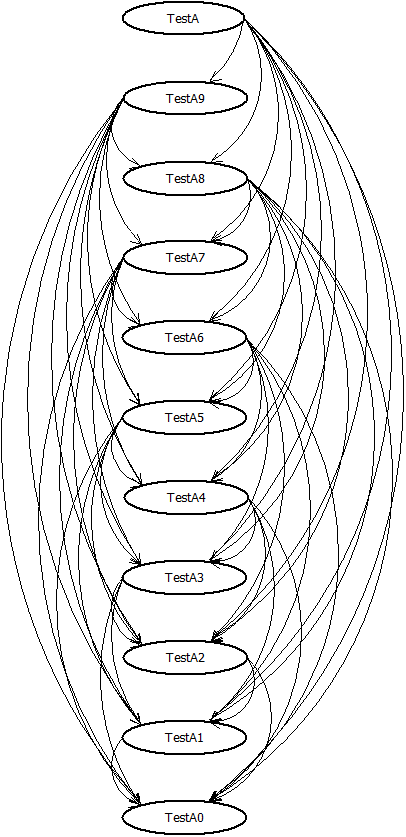
\includegraphics[height=12cm]{TestA.png}
  		\caption{Graf zależności dla testu A.}
  		\label{fig:testA}
	\end{center}
\end{figure}

Łatwo wywnioskować, że tworząc obiekty poszczególnych typów ilość tworzonych obiektów rośnie dwukrotnie:
\begin{itemize}
	\item TestA0 - 1 obiekt,
	\item TestA1 - 2 obiekty (obiekt typu TestA1 i obiekt typu TestA0),
	\item TestA2 - 4 obiekty (obiekt typu TestA2, obiekt typu TestA1 - 2 obiekty, obiekt typu TestA0 - 1 obiekt),
	\item TestA3 - 8 obiektów (obiekt typu TestA3, obiekt typu TestA2 - 4 obiekty, obiekt typu TestA1, obiekt typu TestA0),
	\item TestA4 - 16 obiektów,
	\item TestA5 - 32 obiektów,
	\item TestA6 - 64 obiektów,
	\item TestA7 - 128 obiektów,
	\item TestA8 - 256 obiektów,
	\item TestA9 - 512 obiektów,
	\item TestA - 1 024 obiektów.
\end{itemize}
Zatem tworząc nasz główny obiekt typu TestA, tworzymy: 1 obiekt typu TestA, 1 obiekt typu TestA9, 2 obiekty typu TestA8, 4 obiekty typu TestA7, 8 obiektów typu TestA6, 16 obiektów typu TestA5, 32 obiektów typu TestA4, 64 obiektów typu TestA3, 128 obiektów typu TestA2, 256 obiektów typu TestA1 i 512 obiektów typu TestA0 - co w sumie daje 1024 obiekty.

\subsubsection{Wyniki dla Singleton}
\begin{center}
\begin{small}
	\begin{tabular}{ | l | r r r | r r r | r r r | r r r | }
    		\hline
     		Ilość & & 1 & & & 10 & & & 100 & & & 1000 & \\ \hline
     		 & min & max & avg & min & max & avg & min & max & avg & min & max & avg \\ \hline
    		Autofac & 0 & 0 & 0 & 0 & 0 & 0 & 0 & 0 & 0 & 0 & 0 & 0 \\ \hline
   		DryIoc & 2 & 2 & 2 & 2 & 2 & 2 & 2 & 2 & 2 & 2 & 2 & 2 \\ \hline
		Grace & 2 & 2 & 2 & 2 & 2 & 2 & 2 & 2 & 2 & 2 & 2 & 2 \\ \hline
		LightInject & 2 & 2 & 2 & 2 & 2 & 2 & 2 & 2 & 2 & 2 & 2 & 2 \\ \hline
		Ninject & 3 & 3 & 3 & 3 & 3 & 3 & 3 & 3 & 3 & 6 & 6 & 6 \\ \hline
		NiquIoCPartial & 1 & 1 & 1 & 1 & 1 & 1 & 1 & 1 & 1 & 1 & 1 & 1 \\ \hline
		NiquIoCFull & 2 & 2 & 2 & 2 & 2 & 2 & 2 & 2 & 2 & 2 & 3 & 2 \\ \hline
		SimpleInjector & 2 & 2 & 2 & 2 & 2 & 2 & 2 & 2 & 2 & 2 & 2 & 2 \\ \hline
		StructureMap & 9 & 10 & 9 & 9 & 9 & 9 & 9 & 9 & 9 & 10 & 10 & 10 \\ \hline
		Unity & 7 & 7 & 7 & 7 & 7 & 7 & 7 & 7 & 7 & 8 & 8 & 8 \\ \hline
		Windsor & 0 & 0 & 0 & 0 & 0 & 0 & 0 & 0 & 0 & 0 & 0 & 0 \\
    		\hline
  	\end{tabular}
\end{small}
\end{center}

Najlepiej poradziły sobie najpopularniejsze rozwiązania - Windsor i Aurofac. Rozwiązanie NiquIoCPartial uplasowało się na 3 miejscu. Najsłabiej poradził sobie rozwiązania StructureMap, Unity oraz Ninject.

\subsubsection{Wyniki dla Transient}
\begin{center}
\begin{small}
	\begin{tabular}{ | l | r r r | r r r | r r r | r r r | }
    		\hline
     		Ilość & & 1 & & & 10 & & & 100 & & & 1000 & \\ \hline
     		 & min & max & avg & min & max & avg & min & max & avg & min & max & avg \\ \hline
    		Autofac & 0 & 0 & 0 & 6 & 7 & 6 & 59 & 63 & 60 & 593 & 635 & 602 \\ \hline
		DryIoc & 14 & 14 & 14 & 14 & 15 & 14 & 16 & 16 & 16 & 29 & 29 & 29 \\ \hline
		Grace & 15 & 15 & 15 & 15 & 16 & 15 & 18 & 19 & 18 & 36 & 37 & 36 \\ \hline
		LightInject & 10 & 10 & 10 & 10 & 10 & 10 & 11 & 12 & 11 & 19 & 20 & 19 \\ \hline
		Ninject & 10 & 11 & 10 & 86 & 91 & 87 & 843 & 1089 & 875 & 8585 & 9298 & 8759 \\ \hline
		NiquIoCPartial & 1 & 1 & 1 & 3 & 3 & 3 & 19 & 20 & 19 & 170 & 173 & 171 \\ \hline
		NiquIoCFull & 8 & 8 & 8 & 8 & 8 & 8 & 9 & 10 & 9 & 18 & 19 & 18 \\ \hline
		SimpleInjector & 13 & 14 & 13 & 13 & 14 & 13 & 15 & 15 & 15 & 28 & 29 & 29 \\ \hline
		StructureMap & 10 & 10 & 10 & 13 & 13 & 13 & 53 & 55 & 54 & 415 & 445 & 420 \\ \hline
		Unity & 8 & 8 & 8 & 15 & 15 & 15 & 84 & 86 & 84 & 762 & 765 & 764 \\ \hline
		Windsor & 1 & 1 & 1 & 16 & 18 & 16 & 151 & 156 & 152 & 1504 & 1652 & 1533 \\
    		\hline
  	\end{tabular}
\end{small}
\end{center}
Gdy mamy tylko 1 operację najlepiej radzi sobie Autofac, a zaraz za nim NiquIoCPartial i Windsor. Najsłabiej Grace, DryIoc i SimplyInjector.\\
Dla 10 operacji sytuacja lekko zaczyna się zmieniać. Tym razem znacząco najlepiej radzi sobie NiquIoCPartial (ponad dwa razy lepiej niż drugi Autofac). Kolejne miejsca należą do NiquIoCFull i LightInject. Pozostałe rozwiązania miały podobne, dużo słabsze czasy.Wyjątkiem jest jedynie Ninject, który poradził sobie najgorzej i jego czas jest ponad 5 razy większy niż dla rozwiązania z przedostatnim czasem (Windsor).\\
Gdy mamy 100 operacji na prowadzenie wysuneły się mniej popularne rozwiązania, które prawdopodobniej mają najlepsze cachowanie. Na pierwszym miejscu jest NiquIoCFull, a kolejne miejsca to LightInject i SimpleInjector. Do grona najsłabszym (Ninject, Windsor, Unity) w tym przypadku dołączył również Autofac, który z drugiego miejsca spadł na ósme.\\
Dla przypadku z 1000 operacji do czołówki dołączył DryIoc (czasy zbliżone do SimpleInjector). Na pierwszym miejscu wciąż pozostaje NiquIoCFull, a zaraz za nim LightInject i SimpleInjector. Pozostałe rozwiązania mają czasy od kilka do kilkanaście razy gorsze.\\
Warto tutaj zaznaczyć, że najmniejszy wzorst czasu miały kolejno rozwiązania: LightInject, NiquIoCFull, SimpleInjector, DryIoc oraz Grace.

\subsubsection{Wyniki dla TransientSingleton}
\begin{center}
\begin{small}
	\begin{tabular}{ | l | r r r | r r r | r r r | r r r | }
    		\hline
     		Ilość & & 1 & & & 10 & & & 100 & & & 1000 & \\ \hline
     		 & min & max & avg & min & max & avg & min & max & avg & min & max & avg \\ \hline
    		Autofac & 0 & 0 & 0 & 6 & 6 & 6 & 54 & 56 & 54 & 540 & 566 & 544 \\ \hline
		DryIoc & 18 & 18 & 18 & 19 & 19 & 19 & 20 & 20 & 20 & 31 & 32 & 31 \\ \hline
		Grace & 9 & 9 & 9 & 9 & 10 & 9 & 10 & 11 & 10 & 18 & 18 & 18 \\ \hline
		LightInject & 14 & 14 & 14 & 14 & 14 & 14 & 14 & 14 & 14 & 20 & 20 & 20 \\ \hline
		Ninject & 9 & 10 & 10 & 67 & 73 & 69 & 637 & 678 & 652 & 6426 & 6810 & 6544 \\ \hline
		NiquIoCPartial & 1 & 1 & 1 & 2 & 2 & 2 & 14 & 14 & 14 & 118 & 120 & 118 \\ \hline
		NiquIoCFull & 5 & 5 & 5 & 5 & 6 & 5 & 6 & 6 & 6 & 10 & 11 & 10 \\ \hline
		SimpleInjector & 9 & 9 & 9 & 9 & 10 & 9 & 10 & 10 & 10 & 17 & 17 & 17 \\ \hline
		StructureMap & 9 & 9 & 9 & 12 & 13 & 12 & 35 & 38 & 36 & 252 & 287 & 257 \\ \hline
		Unity & 8 & 8 & 8 & 14 & 14 & 14 & 72 & 72 & 72 & 643 & 650 & 646 \\ \hline
		Windsor & 1 & 1 & 1 & 12 & 12 & 12 & 112 & 129 & 117 & 1108 & 1386 & 1151 \\
    		\hline
  	\end{tabular}
\end{small}
\end{center}
<<opis>>

\subsubsection{Wyniki dla PerThread}
\begin{center}
\begin{small}
	\begin{tabular}{ | l | r r r | r r r | r r r | r r r | }
    		\hline
     		Ilość & & 1 & & & 10 & & & 100 & & & 1000 & \\ \hline
     		 & min & max & avg & min & max & avg & min & max & avg & min & max & avg \\ \hline
    		Autofac & 0 & 0 & 0 & 0 & 0 & 0 & 0 & 0 & 0 & 0 & 0 & 0 \\ \hline
   		DryIoc & 73 & 81 & 76 & 72 & 78 & 75 & 74 & 79 & 76 & 74 & 83 & 77 \\ \hline
		Grace & 4 & 4 & 4 & 4 & 4 & 4 & 4 & 4 & 4 & 4 & 5 & 4 \\ \hline
		LightInject & 51 & 52 & 51 & 51 & 52 & 51 & 51 & 52 & 51 & 51 & 52 & 51 \\ \hline
		Ninject & 3 & 3 & 3 & 3 & 3 & 3 & 3 & 3 & 3 & 6 & 6 & 6 \\ \hline
		NiquIoCPartial & 1 & 1 & 1 & 1 & 1 & 1 & 1 & 1 & 1 & 1 & 1 & 1 \\ \hline
		NiquIoCFull & 2 & 2 & 2 & 2 & 2 & 2 & 2 & 2 & 2 & 2 & 2 & 2 \\ \hline
		SimpleInjector & 7 & 8 & 8 & 7 & 8 & 8 & 7 & 8 & 8 & 8 & 8 & 8 \\ \hline
		StructureMap & 9 & 9 & 9 & 9 & 9 & 9 & 9 & 9 & 9 & 10 & 10 & 10 \\ \hline
		Unity & 7 & 7 & 7 & 7 & 8 & 7 & 7 & 7 & 7 & 8 & 8 & 8 \\ \hline
		Windsor & 0 & 0 & 0 & 0 & 0 & 0 & 0 & 0 & 0 & 0 & 0 & 0 \\
    		\hline
  	\end{tabular}
\end{small}
\end{center}
Czasy dla tego przypadku powinny być zbliżone do czasów dla Singleton, ponieważ wszystko było uruchamiane w jednym wątku. Niestety częć rozwiązań sobie z tym nie poradziła. Czasy zbliżone do czasów dla Singletona posiadają: Autofac, Grace, Ninject, NiquIoCPartial, NiquIoCFull, StructureMap, Unity i Windsor, a dla DryIoC, LightInject i SimpleInjector czasy są od kilka do nawet kilkadziesiąt razy większe.\\
Jeśli chodzi o najlepsze rozwiązania, to wyglądają one tak samo jak dla Singleton - Windso,i Aurofac i NiquIoCPartial. Najsłabiej poradził sobie rozwiązania LightInject i DryIoc. Także w drugiej części tabeli (pod względem czasów) znalazły się Unity, SimpleInjector i StructureMap.


\subsection{Przypadek testowy B}
\subsubsection{Opis}
Ten test jest bardzo podobny do przypadku testowego A, tylko dochodzi nam 1 dodatkowy poziom, który wygląda trochę inaczej. W głównym obiekcie "TestB" konstruktor przyjmuje 3 parametry następujących typów: "TestBa10", "TestBb10", "TestBc10". Każdy z tych 3 typów odpowiada typowi "TestA", więc przyjmuje on w konstruktorze 10 parametrów. Dla "TestBa10" są to parametry typów od "TestBa0" do "TestBa9", dla "TestBb10" są to parametry typów od "TestBb0" do "TestBb9", a dla "TestBc10" są to parametry typów od "TestBc0" do "TestBc9". Zależności tych typów wyglądają tak samo, jak dla typów z przypadku testowego A - rys. \ref{fig:testB} przedstawia te zależności. \\

\clearpage
\begin{figure}[h]
	\begin{center}
  		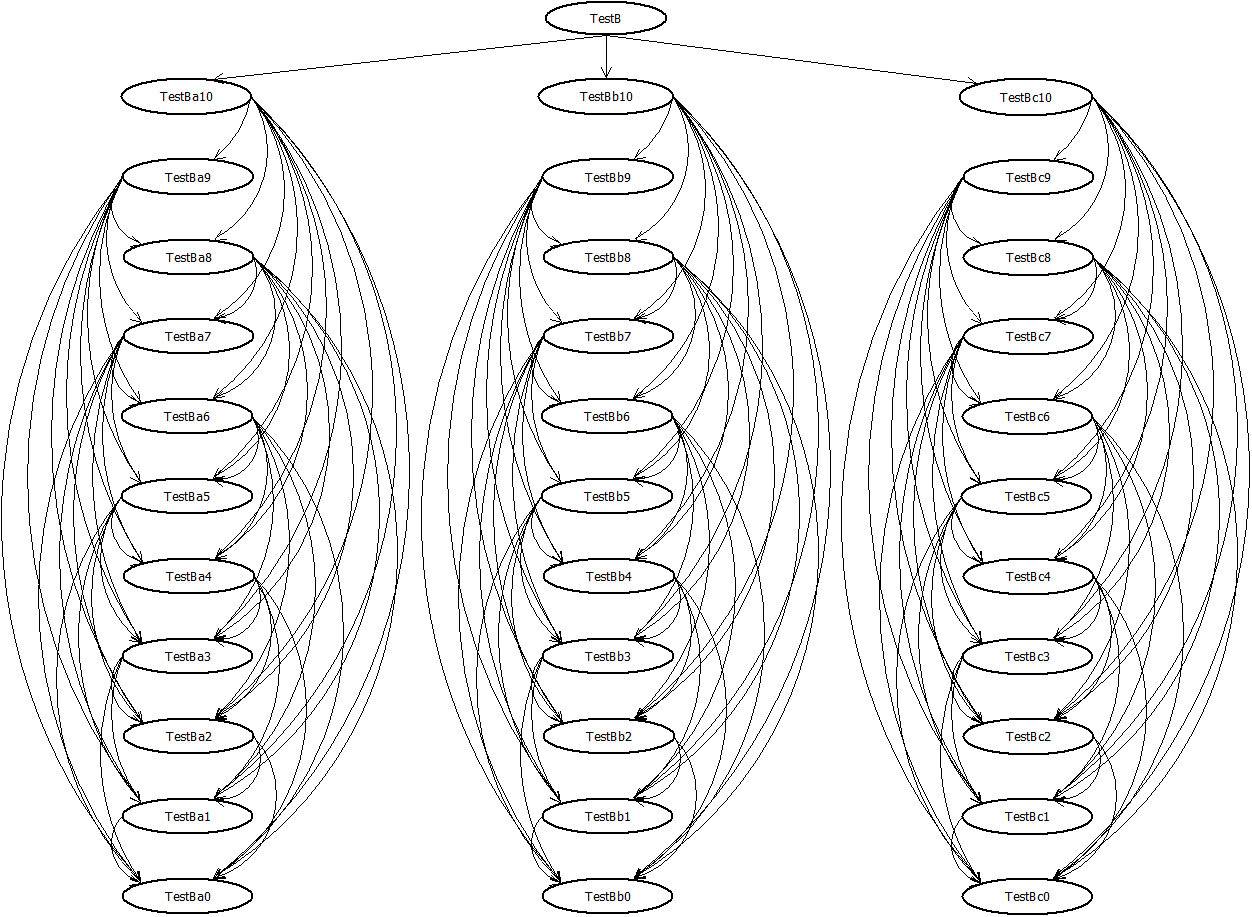
\includegraphics[width=\linewidth]{TestB.png}
  		\caption{Graf zależności dla testu B.}
  		\label{fig:testB}
	\end{center}
\end{figure}

Łatwo wywnioskować, że tworząc obiekty poszczególnych typów ilość tworzonych obiektów rośnie dwukrotnie (tak jak dla testu A):
\begin{itemize}
	\item TestBa0 - 1 obiekt,
	\item TestBa1 - 2 obiekty (obiekt typu TestBa1 i obiekt typu TestBa0),
	\item TestBa2 - 4 obiekty (obiekt typu TestBa2, obiekt typu TestBa1 - 2 obiekty, obiekt typu TestBa0 - 1 obiekt),
	\item TestBa3 - 8 obiektów (obiekt typu TestBa3, obiekt typu TestBa2 - 4 obiekty, obiekt typu TestBa1, obiekt typu TestBa0),
	\item TestBa4 - 16 obiektów,
	\item TestBa5 - 32 obiektów,
	\item TestBa6 - 64 obiektów,
	\item TestBa7 - 128 obiektów,
	\item TestBa8 - 256 obiektów,
	\item TestBa9 - 512 obiektów,
	\item TestBa10 - 1 024 obiektów,
	\item \ldots (dla TestBb i TestBc sytuacja wygląda dokłądnie tak samo jak dla TestBa),
	\item TestB - 3 073 obiektów.
\end{itemize}
Zatem tworząc obiekt typu TestB, tworzymy: 1 obiekt typu TestB, 1 obiekt typu TestBa10, TestBb10 i TestBc10,1 obiekt typu TestBa9, TestBb9 i TestBc9, 2 obiekty typu TestBa8, TestBb8 i TestBc8, 4 obiekty typu TestBa7, TestBb7 i TestBc7, 8 obiektów typu TestBa6, TestBb6 i TestBc6, 16 obiektów typu TestBa5, TestBb5 i TestBc5, 32 obiektów typu TestBa4, TestBb4 i TestBc4, 64 obiektów typu TestBa3, TestBb3 i TestBc3, 128 obiektów typu TestBa2, TestBb2 i TestBc2, 256 obiektów typu TestBa1, TestBb1 i TestBc1, 512 obiektów typu TestBa0, TestBb0 i TestBc0 - co daje w sumie 3 073 obiektów.

\subsubsection{Wyniki dla Singleton}
\begin{center}
\begin{small}
	\begin{tabular}{ | l | r r r | r r r | r r r | r r r | }
    		\hline
     		Ilość & & 1 & & & 10 & & & 100 & & & 1000 & \\ \hline
     		 & min & max & avg & min & max & avg & min & max & avg & min & max & avg \\ \hline
    		Autofac & 0 & 0 & 0 & 0 & 0 & 0 & 0 & 0 & 0 & 0 & 0 & 0 \\ \hline
   		DryIoc & 8 & 9 & 8 & 8 & 9 & 9 & 8 & 9 & 9 & 8 & 9 & 8 \\ \hline
		Grace & 8 & 8 & 8 & 8 & 8 & 8 & 8 & 8 & 8 & 8 & 8 & 8 \\ \hline
		LightInject & 6 & 7 & 6 & 6 & 7 & 6 & 6 & 6 & 6 & 6 & 7 & 6 \\ \hline
		Ninject & 9 & 9 & 9 & 9 & 9 & 9 & 9 & 10 & 9 & 12 & 13 & 12 \\ \hline
		NiquIoCPartial & 4 & 4 & 4 & 4 & 4 & 4 & 4 & 4 & 4 & 4 & 4 & 4 \\ \hline
		NiquIoCFull & 8 & 8 & 8 & 8 & 8 & 8 & 8 & 8 & 8 & 8 & 8 & 8 \\ \hline
		SimpleInjector & 6 & 6 & 6 & 6 & 6 & 6 & 6 & 6 & 6 & 6 & 6 & 6 \\ \hline
		StructureMap & 30 & 30 & 30 & 30 & 30 & 30 & 30 & 30 & 30 & 32 & 33 & 33 \\ \hline
		Unity & 23 & 23 & 23 & 23 & 23 & 23 & 23 & 23 & 23 & 24 & 24 & 24 \\ \hline
		Windsor & 0 & 0 & 0 & 0 & 0 & 0 & 0 & 0 & 0 & 0 & 0 & 0 \\
    		\hline
  	\end{tabular}
\end{small}
\end{center}
Dla tego przypadku testowego również najlepiej poradziły sobie najpopularniejsze rozwiązania - Aurofac i Windso. Kontener NiquIoCPartial uplasował się tutaj również na 3 miejscu. Najsłabiej poradził sobie rozwiązania StructureMap, Unity oraz Ninject.

\subsubsection{Wyniki dla Transient}
\begin{center}
\begin{small}
	\begin{tabular}{ | l | r r r | r r r | r r r | r r r | }
    		\hline
     		Ilość & & 1 & & & 10 & & & 100 & & & 1000 & \\ \hline
     		 & min & max & avg & min & max & avg & min & max & avg & min & max & avg \\ \hline
    		Autofac & 2 & 2 & 2 & 21 & 23 & 22 & 194 & 218 & 204 & 1972 & 2043 & 2008 \\ \hline
		DryIoc & 44 & 46 & 45 & 45 & 46 & 45 & 52 & 55 & 53 & 100 & 104 & 102 \\ \hline
		Grace & 51 & 52 & 51 & 52 & 53 & 52 & 58 & 59 & 58 & 123 & 126 & 124 \\ \hline
		LightInject & 32 & 32 & 32 & 32 & 33 & 32 & 37 & 39 & 37 & 71 & 72 & 72 \\ \hline
		Ninject & 35 & 42 & 36 & 271 & 297 & 277 & 2697 & 3014 & 2787 & 27790 & 28442 & 28038 \\ \hline
		NiquIoCPartial & 5 & 5 & 5 & 10 & 10 & 10 & 57 & 58 & 58 & 522 & 529 & 524 \\ \hline
		NiquIoCFull & 26 & 32 & 27 & 26 & 27 & 26 & 32 & 33 & 32 & 66 & 67 & 66 \\ \hline
		SimpleInjector & 40 & 40 & 40 & 40 & 41 & 41 & 46 & 47 & 47 & 94 & 95 & 94 \\ \hline
		StructureMap & 33 & 33 & 33 & 44 & 45 & 45 & 162 & 165 & 163 & 1296 & 1364 & 1311 \\ \hline
		Unity & 27 & 28 & 28 & 48 & 50 & 49 & 257 & 265 & 258 & 2324 & 2334 & 2329 \\ \hline
		Windsor & 6 & 6 & 6 & 48 & 64 & 50 & 466 & 498 & 474 & 4627 & 4893 & 4702 \\
    		\hline
  	\end{tabular}
\end{small}
\end{center}
Gdy mamy tylko 1 operację najlepiej radzi sobie Autofac, a zaraz za nim NiquIoCPartial i Windsor. Najsłabiej DryIoc i SimplyInjector.\\
Gdy mamy 10 operacji znacząco lepiej niż reszta radzi sobie NiquIoCPartial - czasy ponad dwa mniejsze niż dla zajmującego drugie Autofac. Kolejne miejsca należą do NiquIoCFull i LightInject. Pozostałe rozwiązania miałby podobne, trochę słabsze czasy. Najgorzej poradził sobie Ninject, który czas miał ponad 5 razy większy niż rozwiązanie z przedostatnim czasem (Grace).\\
Tutaj również gdy mamy 100 operacji na prowadzenie wysuneły się mniej popularne rozwiązania. Kolejne miejsca to: NiquIoCFull, LightInject i SimpleInjector. Najsłabiej w tym przypadku poradziłysobie Ninject, Windsor, Unity i Autofac. Grace w 9 miejsca od końca awansował na 6, a NiquIoCPartial z pierwszego spadł na 5.\\
Dla przypadku z 1000 operacji do czołówki dołączył DryIoc i Grace - czasy trochę słabsze niż SimpleInjector. Pierwsze trzy miejsca nie uległu zmianie.\\
Tutaj najmniejszy wzorst czasu miały rozwiążania: NiquIoCFull, LightInject, SimpleInjector, DryIoc oraz Grace.

\subsubsection{Wyniki dla TransientSingleton}
\begin{center}
\begin{small}
	\begin{tabular}{ | l | r r r | r r r | r r r | r r r | }
    		\hline
     		Ilość & & 1 & & & 10 & & & 100 & & & 1000 & \\ \hline
     		 & min & max & avg & min & max & avg & min & max & avg & min & max & avg \\ \hline
    		Autofac & 1 & 1 & 1 & 18 & 19 & 18 & 175 & 179 & 176 & 1732 & 1806 & 1751 \\ \hline
		DryIoc & 56 & 56 & 56 & 57 & 57 & 57 & 63 & 64 & 63 & 107 & 108 & 108 \\ \hline
		Grace & 30 & 30 & 30 & 30 & 30 & 30 & 34 & 35 & 34 & 67 & 68 & 68 \\ \hline
		LightInject & 47 & 48 & 48 & 48 & 49 & 48 & 50 & 52 & 51 & 80 & 80 & 80 \\ \hline
		Ninject & 29 & 31 & 30 & 214 & 220 & 217 & 2016 & 2102 & 2045 & 20354 & 21113 & 20622 \\ \hline
		NiquIoCPartial & 4 & 5 & 5 & 8 & 8 & 8 & 42 & 42 & 42 & 369 & 371 & 369 \\ \hline
		NiquIoCFull & 16 & 16 & 16 & 16 & 16 & 16 & 18 & 20 & 18 & 37 & 38 & 37 \\ \hline
		SimpleInjector & 27 & 28 & 28 & 28 & 28 & 28 & 32 & 33 & 32 & 60 & 62 & 61 \\ \hline
		StructureMap & 32 & 33 & 32 & 39 & 40 & 39 & 111 & 118 & 113 & 795 & 805 & 800 \\ \hline
		Unity & 27 & 28 & 28 & 46 & 47 & 46 & 225 & 228 & 227 & 2010 & 2025 & 2018 \\ \hline
		Windsor & 3 & 4 & 3 & 35 & 36 & 35 & 338 & 395 & 348 & 3368 & 3589 & 3416 \\
    		\hline
  	\end{tabular}
\end{small}
\end{center}
<<opis>>

\subsubsection{Wyniki dla PerThread}
\begin{center}
\begin{small}
	\begin{tabular}{ | l | r r r | r r r | r r r | r r r | }
    		\hline
     		Ilość & & 1 & & & 10 & & & 100 & & & 1000 & \\ \hline
     		 & min & max & avg & min & max & avg & min & max & avg & min & max & avg \\ \hline
    		Autofac & 0 & 0 & 0 & 0 & 0 & 0 & 0 & 0 & 0 & 0 & 0 & 0 \\ \hline
   		DryIoc & 247 & 260 & 252 & 247 & 257 & 250 & 247 & 271 & 255 & 256 & 272 & 263 \\ \hline
		Grace & 13 & 13 & 13 & 13 & 13 & 13 & 13 & 13 & 13 & 13 & 13 & 13 \\ \hline
		LightInject & -1 & -1 & -1 & -1 & -1 & -1 & -1 & -1 & -1 & -1 & -1 & -1 \\ \hline
		Ninject & 9 & 9 & 9 & 9 & 9 & 9 & 9 & 10 & 9 & 12 & 13 & 12 \\ \hline
		NiquIoCPartial & 4 & 4 & 4 & 4 & 4 & 4 & 4 & 4 & 4 & 4 & 4 & 4 \\ \hline
		NiquIoCFull & 8 & 8 & 8 & 8 & 8 & 8 & 8 & 8 & 8 & 8 & 8 & 8 \\ \hline
		SimpleInjector & 23 & 23 & 23 & 23 & 23 & 23 & 23 & 23 & 23 & 23 & 23 & 23 \\ \hline
		StructureMap & 30 & 30 & 30 & 30 & 30 & 30 & 30 & 30 & 30 & 32 & 33 & 33 \\ \hline
		Unity & 23 & 23 & 23 & 23 & 23 & 23 & 23 & 23 & 23 & 24 & 24 & 24 \\ \hline
		Windsor & 0 & 0 & 0 & 0 & 0 & 0 & 0 & 0 & 0 & 0 & 0 & 0 \\
    		\hline
  	\end{tabular}
\end{small}
\end{center}
Tutaj również nie wszystkie rozwiązania mają czasy zbliżone do Singleton. Są to te same rozwiązania co dla przypadku testowego B, czyli: DryIoc, Grace, LightInject, SimpleInjector.\\
Tak samo jak w przypadku Signleton czołówka wygląda następująco: Aurofac, Windsor i NiquIoCPartial. Kolejne miejsca to NiquIoCFull, Ninject i Grace. Najsłabiej poradził sobie rozwiążania LightInject i DryIoc.


\subsection{Przypadek testowy C}
\subsubsection{Opis}
W tym teście mamy zdefiniowanych 26 typów. 5 z tych typów ma konstruktor bezparametrowy, a pozostałe 21 ma konstuktor z pięcioma parametrami. Typem głównym jest typ "TestC". Obiekt tego typy w konstruktorze przymuje 5 innych obiektów, kolejno następujących typów: "TestC40", "TestC41", "TestC42", "TestC43" i "TestC44". Każdy z tych pięciu typów ma taki sam konstruktor - przyjmuje w nim 5 obiektów o typach z pierwszym numerkiem o 1 mniejszym (czyli przyjmują w konstruktorze obiekty typów od "TestC30" do "TestC34"). Dla typów od "TestC30" do "TestC34" zasad z konstruktorami wygląda tak samo. Na końcu dochodzimy do typów od "TestC00" do "TestC04", które mają konstruktor bezparametrowy. Rys. \ref{fig:testC} przedstawia graf zależności typów dla tego przypadku testowego.

\begin{figure}[h]
	\begin{center}
  		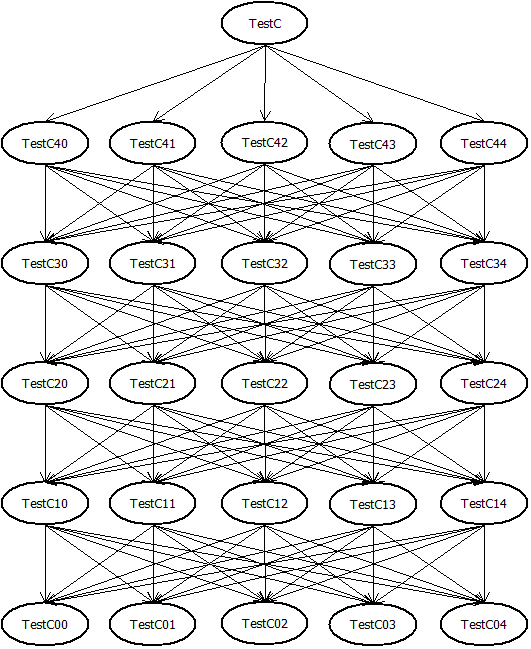
\includegraphics[height=10cm]{TestC.png}
  		\caption{Graf zależności dla testu C.}
  		\label{fig:testC}
	\end{center}
\end{figure}

Łatwo wywnioskować, że tworząc obiekty poszczególnych typów ilość tworzonych obiektów rośnie ponad dziesięciokortnie:
\begin{itemize}
	\item typy od TestC00 do TestC04 - 1 obiekt,
	\item typy od TestC10 do TestC14 - 6 obiektów (obiekt danego typu plus 5 obiektów typów od TestC00 do TestC04),
	\item typy od TestC20 do TestC24 - 31 obiektów (obiekt danego typu plus 5 obiektów typów od TestC10 do TestC14),
	\item typy od TestC30 do TestC34 - 156 obiektów,
	\item  typy od TestC40 do TestC44 - 781 obiektów,
	\item TestC - 3 906 obiektów.
\end{itemize}
Zatem tworząc obiekt typu TestC, tworzymy: 1 obiekt typu TestC, 5 obiektów typów od TestC40 do TestC44, 25 obiektów typów od TestC30 do TestC34, 125 obiektów typów od TestC20 do TestC24, 625 obiektów typów od TestC10 do TestC14, 3 125 obiektów typów od TestC00 do TestC04 - co daje w sumie 3 906 obiektów.

\subsubsection{Wyniki dla Singleton}
\begin{center}
\begin{small}
	\begin{tabular}{ | l | r r r | r r r | r r r | r r r | }
    		\hline
     		Ilość & & 1 & & & 10 & & & 100 & & & 1000 & \\ \hline
     		 & min & max & avg & min & max & avg & min & max & avg & min & max & avg \\ \hline
    		Autofac & 0 & 0 & 0 & 0 & 0 & 0 & 0 & 0 & 0 & 0 & 0 & 0 \\ \hline
		DryIoc & 5 & 5 & 5 & 5 & 5 & 5 & 5 & 5 & 5 & 5 & 5 & 5 \\ \hline
		Grace & 5 & 5 & 5 & 5 & 5 & 5 & 5 & 5 & 5 & 5 & 5 & 5 \\ \hline
		LightInject & 4 & 4 & 4 & 4 & 4 & 4 & 4 & 4 & 4 & 4 & 4 & 4 \\ \hline
		Ninject & 6 & 6 & 6 & 6 & 6 & 6 & 6 & 7 & 6 & 9 & 10 & 9 \\ \hline
		NiquIoCPartial & 3 & 3 & 3 & 3 & 3 & 3 & 3 & 3 & 3 & 3 & 3 & 3 \\ \hline
		NiquIoCFull & 5 & 6 & 5 & 5 & 5 & 5 & 5 & 5 & 5 & 5 & 6 & 5 \\ \hline
		SimpleInjector & 4 & 4 & 4 & 4 & 4 & 4 & 4 & 4 & 4 & 4 & 4 & 4 \\ \hline
		StructureMap & 22 & 22 & 22 & 22 & 22 & 22 & 22 & 22 & 22 & 23 & 23 & 23 \\ \hline
		Unity & 15 & 16 & 15 & 15 & 16 & 15 & 15 & 16 & 16 & 16 & 16 & 16 \\ \hline
		Windsor & 0 & 0 & 0 & 0 & 0 & 0 & 0 & 0 & 0 & 0 & 0 & 0 \\
    		\hline
  	\end{tabular}
\end{small}
\end{center}
<<opis>>

\subsubsection{Wyniki dla Transient}
\begin{center}
\begin{small}
	\begin{tabular}{ | l | r r r | r r r | r r r | r r r | }
    		\hline
     		Ilość & & 1 & & & 10 & & & 100 & & & 1000 & \\ \hline
     		 & min & max & avg & min & max & avg & min & max & avg & min & max & avg \\ \hline
    		Autofac & 2 & 2 & 2 & 24 & 25 & 24 & 234 & 240 & 235 & 2315 & 2330 & 2322 \\ \hline
		DryIoc & 39 & 39 & 39 & 40 & 40 & 40 & 47 & 48 & 47 & 98 & 99 & 98 \\ \hline
		Grace & 60 & 61 & 61 & 61 & 64 & 62 & 72 & 73 & 72 & 150 & 155 & 151 \\ \hline
		LightInject & 36 & 37 & 36 & 36 & 37 & 37 & 43 & 44 & 44 & 86 & 86 & 86 \\ \hline
		Ninject & 38 & 40 & 38 & 343 & 354 & 348 & 3386 & 3498 & 3432 & 36355 & 37506 & 36938 \\ \hline
		NiquIoCPartial & 3 & 4 & 3 & 10 & 10 & 10 & 71 & 72 & 71 & 676 & 683 & 678 \\ \hline
		NiquIoCFull & 31 & 33 & 31 & 31 & 33 & 32 & 38 & 38 & 38 & 81 & 86 & 84 \\ \hline
		SimpleInjector & 40 & 41 & 40 & 41 & 42 & 41 & 49 & 49 & 49 & 113 & 114 & 114 \\ \hline
		StructureMap & 26 & 26 & 26 & 40 & 40 & 40 & 179 & 182 & 180 & 1530 & 1553 & 1542 \\ \hline
		Unity & 19 & 19 & 19 & 47 & 49 & 47 & 311 & 351 & 316 & 2954 & 3069 & 2974 \\ \hline
		Windsor & 6 & 7 & 7 & 59 & 75 & 61 & 575 & 585 & 581 & 5755 & 6318 & 5846 \\
    		\hline
  	\end{tabular}
\end{small}
\end{center}
<<opis>>

\subsubsection{Wyniki dla TransientSingleton}
\begin{center}
\begin{small}
	\begin{tabular}{ | l | r r r | r r r | r r r | r r r | }
    		\hline
     		Ilość & & 1 & & & 10 & & & 100 & & & 1000 & \\ \hline
     		 & min & max & avg & min & max & avg & min & max & avg & min & max & avg \\ \hline
    		Autofac & 1 & 2 & 1 & 19 & 20 & 19 & 182 & 188 & 184 & 1790 & 1827 & 1806 \\ \hline
		DryIoc & 58 & 58 & 58 & 59 & 107 & 64 & 64 & 65 & 64 & 104 & 106 & 105 \\ \hline
		Grace & 22 & 22 & 22 & 22 & 23 & 22 & 25 & 25 & 25 & 43 & 44 & 44 \\ \hline
		LightInject & 52 & 52 & 52 & 52 & 54 & 52 & 55 & 55 & 55 & 82 & 84 & 83 \\ \hline
		Ninject & 26 & 28 & 27 & 199 & 219 & 204 & 1908 & 2017 & 1938 & 19238 & 20310 & 19572 \\ \hline
		NiquIoCPartial & 3 & 3 & 3 & 6 & 7 & 6 & 38 & 38 & 38 & 337 & 346 & 341 \\ \hline
		NiquIoCFull & 12 & 13 & 12 & 12 & 12 & 12 & 13 & 14 & 13 & 25 & 25 & 25 \\ \hline
		SimpleInjector & 21 & 21 & 21 & 21 & 21 & 21 & 23 & 24 & 23 & 44 & 44 & 44 \\ \hline
		StructureMap & 22 & 22 & 22 & 29 & 29 & 29 & 79 & 80 & 80 & 546 & 549 & 547 \\ \hline
		Unity & 18 & 18 & 18 & 39 & 40 & 40 & 240 & 242 & 241 & 2246 & 2372 & 2268 \\ \hline
		Windsor & 3 & 3 & 3 & 32 & 33 & 33 & 319 & 383 & 328 & 3162 & 3316 & 3195 \\
    		\hline
  	\end{tabular}
\end{small}
\end{center}
<<opis>>

\subsubsection{Wyniki dla PerThread}
\begin{center}
\begin{small}
	\begin{tabular}{ | l | r r r | r r r | r r r | r r r | }
    		\hline
     		Ilość & & 1 & & & 10 & & & 100 & & & 1000 & \\ \hline
     		 & min & max & avg & min & max & avg & min & max & avg & min & max & avg \\ \hline
    		Autofac & 0 & 0 & 0 & 0 & 0 & 0 & 0 & 0 & 0 & 0 & 0 & 0 \\ \hline
		DryIoc & 155 & 156 & 155 & 155 & 155 & 155 & 155 & 157 & 155 & 155 & 156 & 156 \\ \hline
		Grace & 8 & 8 & 8 & 8 & 8 & 8 & 8 & 8 & 8 & 8 & 8 & 8 \\ \hline
		LightInject & 523 & 541 & 526 & 523 & 529 & 526 & 523 & 527 & 525 & 523 & 528 & 527 \\ \hline
		Ninject & 6 & 7 & 6 & 6 & 6 & 6 & 6 & 7 & 6 & 9 & 10 & 9 \\ \hline
		NiquIoCPartial & 3 & 3 & 3 & 3 & 3 & 3 & 3 & 3 & 3 & 3 & 3 & 3 \\ \hline
		NiquIoCFull & 5 & 5 & 5 & 5 & 5 & 5 & 5 & 5 & 5 & 5 & 5 & 5 \\ \hline
		SimpleInjector & 15 & 16 & 16 & 15 & 16 & 16 & 15 & 16 & 16 & 16 & 16 & 16 \\ \hline
		StructureMap & 22 & 22 & 22 & 22 & 22 & 22 & 22 & 22 & 22 & 23 & 23 & 23 \\ \hline
		Unity & 15 & 16 & 15 & 15 & 16 & 16 & 15 & 16 & 16 & 16 & 16 & 16 \\ \hline
		Windsor & 0 & 0 & 0 & 0 & 0 & 0 & 0 & 0 & 0 & 0 & 0 & 0 \\
    		\hline
  	\end{tabular}
\end{small}
\end{center}
<<opis>>


\subsection{Przypadek testowy D}
\subsubsection{Opis}
W tym teście mamy zdefiniowanych 51 typów. 10 z tych typów ma konstruktor bezparametrowy, a pozostałe 41 ma konstuktor z dziesięcioma parametrami. Typem głównym jest typ "TestD". Obiekt tego typy w konstruktorze przymuje 10 innych obiektów, kolejno następujących typów: "TestD40", "TestD41", "TestD42", "TestD43", "TestD44", "TestD45", "TestD46", "TestD47", "TestD48", "TestD49". Każdy z tych 10 typów w konstruktorze przyjmuje 10 obiektów o takich samych typach, ale z pierwszym numerkiem o 1 mniejszym (czyli obiekty typów od "TestD40" do "TestD49", przyjmują w konstruktorze obiekty typów od "TestD30" do "TestD39"). Dla typów od "TestD30" do "TestD39" zasad z konstruktorami wygląda tak samo. Na końcu dochodzimy do typów od "TestD00" do "TestD09", które mają konstruktor bezparametrowy. Rys. \ref{fig:testD} przedstawia graf zależności typów dla tego przypadku testowego.

\begin{figure}[h]
	\begin{center}
  		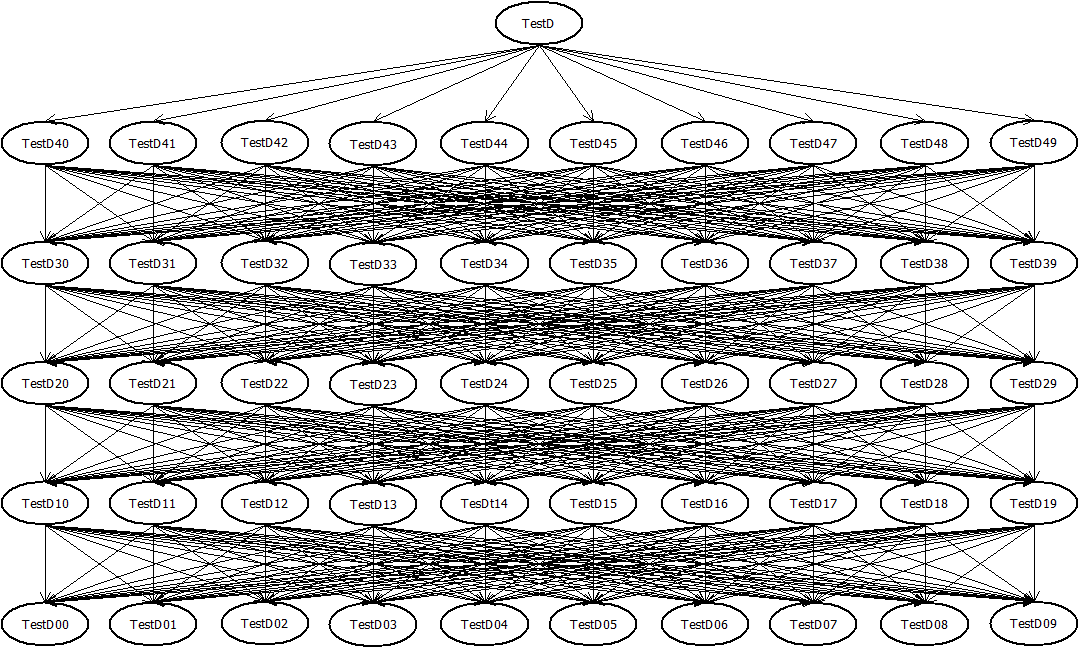
\includegraphics[width=\linewidth]{TestD.png}
  		\caption{Graf zależności dla testu D.}
  		\label{fig:testD}
	\end{center}
\end{figure}

Łatwo wywnioskować, że tworząc obiekty poszczególnych typów ilość tworzonych obiektów rośnie ponad dziesięciokortnie:
\begin{itemize}
	\item typy od TestD00 do TestD09 - 1 obiekt,
	\item typy od TestD10 do TestD19 - 11 obiektów (obiekt danego typu plus 10 obiektów typów od TestD00 do TestD09),
	\item typy od TestD20 do TestD29 - 111 obiektów (obiekt danego typu plus 10 obiektów typów od TestD10 do TestD19),
	\item typy od TestD30 do TestD39 - 1 111 obiektów,
	\item  typy od TestD40 do TestD49 - 11 111 obiektów,
	\item TestD - 111 111 obiektów.
\end{itemize}
Zatem tworząc obiekt typu TestD, tworzymy: 1 obiekt typu TestD, 10 obiektów typów od TestD40 do TestD49, 100 obiektów typów od TestD30 do TestD39, 1 000 obiektów typów od TestD20 do TestD29, 10 000 obiektów typów od TestD10 do TestD19, 100 000 obiektów typów od TestD00 do TestD09 - co daje w sumie 111 111 obiektów..

\subsubsection{Wyniki dla Singleton}
\begin{center}
\begin{small}
	\begin{tabular}{ | l | r r r | r r r | }
    		\hline
     		Ilość & & 1 & & & 10 &  \\ \hline
     		 & min & max & avg & min & max & avg \\ \hline
		Autofac & 0 & 0 & 0 & 0 & 0 & 0 \\ \hline
		DryIoc & 10 & 11 & 10 & 10 & 13 & 10 \\ \hline
		Grace & 17 & 20 & 18 & 17 & 18 & 18 \\ \hline
		LightInject & 14 & 14 & 14 & 14 & 14 & 14 \\ \hline
		Ninject & 21 & 21 & 21 & 21 & 22 & 21 \\ \hline
		NiquIoCPartial & 8 & 9 & 9 & 8 & 9 & 9 \\ \hline
		NiquIoCFull & 18 & 18 & 18 & 18 & 18 & 18 \\ \hline
		SimpleInjector & 11 & 12 & 11 & 11 & 12 & 11 \\ \hline
		StructureMap & 51 & 51 & 51 & 51 & 51 & 51 \\ \hline
		Unity & 51 & 52 & 52 & 51 & 52 & 52 \\ \hline
		Windsor & 0 & 0 & 0 & 0 & 0 & 0 \\
    		\hline
  	\end{tabular}
\end{small}
\end{center}
Podobnie jak dla przypadku testowego A, tutaj również najlepiej poradziły sobie najpopularniejsze rozwiązania - Windsor i Aurofac. Na trzecim miejscu znajduje się rozwiązanie NiquIoCPartial. Najsłabiej poradził sobie rozwiązania StructureMap i Unity.

\subsubsection{Wyniki dla Transient}
\begin{center}
\begin{small}
	\begin{tabular}{ | l | r r r | r r r | }
    		\hline
     		Ilość & & 1 & & & 10 &  \\ \hline
     		 & min & max & avg & min & max & avg \\ \hline
		Autofac & 145 & 169 & 156 & 1302 & 1352 & 1318 \\ \hline
		DryIoc & 1038 & 1086 & 1062 & 1068 & 1101 & 1089 \\ \hline
		Grace & 1480 & 1553 & 1507 & 1511 & 1586 & 1551 \\ \hline
		LightInject & 818 & 839 & 831 & 870 & 878 & 873 \\ \hline
		Ninject & 1039 & 1189 & 1068 & 10104 & 10604 & 10299 \\ \hline
		NiquIoCPartial & 36 & 37 & 36 & 284 & 304 & 289 \\ \hline
		NiquIoCFull & 568 & 573 & 570 & 628 & 651 & 635 \\ \hline
		SimpleInjector & 175 & 176 & 175 & 203 & 204 & 204 \\ \hline
		StructureMap & 104 & 106 & 105 & 580 & 635 & 588 \\ \hline
		Unity & 149 & 151 & 150 & 1069 & 1089 & 1074 \\ \hline
		Windsor & 176 & 204 & 181 & 1777 & 1800 & 1785 \\
    		\hline
  	\end{tabular}
\end{small}
\end{center}
Dla tego testu rozbierzność czasów jest dość duża.\\
Gdy mamy tylko 1 operację najlepiej radzi sobie NiquIoCPartial. Czasy pozostały są znacząco większe. Najsłabiej poradziły sobie Grace, Ninject, DryIoc i LightInject.\\
Dla 10 operacji znacząco najlepiej radzi sobie SimplyInjector i NiquIoCPartial. Czołówkę zamykają StrucutreMap i NiquIoCFull. Pozostałe rozwiązania miały podobne, dużo słabsze czasy. Wyjątkiem jest ponownie Ninject, którego czasy są kilkukrotnie większe.\\
W tym przypadku najmniejszy wzorst czasu miały kolejno rozwiązania: DryIoc, SimpleInjector, LightInject, Grace oraz NiquIoCFull.

\subsubsection{Wyniki dla TransientSingleton}
\begin{center}
\begin{small}
	\begin{tabular}{ | l | r r r | r r r | }
    		\hline
     		Ilość & & 1 & & & 10 &  \\ \hline
     		 & min & max & avg & min & max & avg \\ \hline
		Autofac & 77 & 78 & 77 & 898 & 917 & 904 \\ \hline
		DryIoc & 891 & 896 & 893 & 921 & 959 & 928 \\ \hline
		Grace & 362 & 369 & 364 & 369 & 378 & 371 \\ \hline
		LightInject & 1278 & 1368 & 1303 & 1290 & 1332 & 1303 \\ \hline
		Ninject & 511 & 561 & 524 & 4824 & 5067 & 4881 \\ \hline
		NiquIoCPartial & 17 & 17 & 17 & 100 & 101 & 101 \\ \hline
		NiquIoCFull & 143 & 144 & 143 & 150 & 158 & 154 \\ \hline
		SimpleInjector & 85 & 86 & 85 & 90 & 91 & 90 \\ \hline
		StructureMap & 60 & 66 & 61 & 166 & 169 & 167 \\ \hline
		Unity & 116 & 117 & 116 & 693 & 699 & 695 \\ \hline
		Windsor & 83 & 89 & 85 & 832 & 918 & 853 \\
    		\hline
  	\end{tabular}
\end{small}
\end{center}
<<opis>>

\subsubsection{Wyniki dla PerThread}
\begin{center}
\begin{small}
	\begin{tabular}{ | l | r r r | r r r | }
    		\hline
     		Ilość & & 1 & & & 10 &  \\ \hline
     		 & min & max & avg & min & max & avg \\ \hline
		Autofac & 0 & 0 & 0 & 0 & 0 & 0 \\ \hline
		DryIoc & 1062 & 1126 & 1093 & 1078 & 1117 & 1097 \\ \hline
		Grace & 28 & 28 & 28 & 28 & 28 & 28 \\ \hline
		LightInject & -1 & -1 & -1 & -1 & -1 & -1 \\ \hline
		Ninject & 21 & 21 & 21 & 21 & 22 & 21 \\ \hline
		NiquIoCPartial & 8 & 9 & 9 & 8 & 9 & 9 \\ \hline
		NiquIoCFull & 18 & 18 & 18 & 18 & 18 & 18 \\ \hline
		SimpleInjector & 46 & 46 & 46 & 46 & 47 & 46 \\ \hline
		StructureMap & 51 & 51 & 51 & 51 & 51 & 51 \\ \hline
		Unity & 51 & 53 & 52 & 51 & 52 & 52 \\ \hline
		Windsor & 0 & 0 & 0 & 0 & 0 & 0 \\
    		\hline
  	\end{tabular}
\end{small}
\end{center}
Tutaj tak samo jak dla przypadku testowego A czasy powinny być zbliżone do czasów dla Singleton. Niestety dla tego testu również nie wszystkie rozwiązania sobie z tym poradziły. Dużo słabsze czasy niż w przypadku Singleton miały rozwiązania: DryIoc, Grace, LightInject, SimpleInjector.\\
Zarówno dla 1 jak i 10 powtórzeń najlepiej radzi sobie Autofac i Windsor. Podium ponownie zamyka NiquIoCPartial.\\
Najgorzej poradził sobie tutaj LightInject, który trwał ponad 20 minut (stąd w rozwiążaniu czas "-1"). DryIoc również poradził sobie bardzo słabo - czasy ponad 20 raz gorsze niż rozwiążanie na miejscu o 1 wyższym (Unity).


\clearpage

\section{Podsumowanie}
<parę słów na koniec>

\newpage
\begin{thebibliography}{authordate1}
\bibitem{dependency_injection} Mark Seemann, Dependency Injection in .NET, 2012
\bibitem{emit} Serge Lidin, Expert .NET 2.0 IL Assembler, 2006
\end{thebibliography}

\end{document}